\documentclass[12pt,a4paper]{article} 
\usepackage{graphicx}
\linespread{1.5}
\begin{document}
\title{Instalasi PIP dan Contoh Penggunaan}
\maketitle

\begin{itemize}
\item
Nama Kelompok 1\\
Farid Ariyanto Saputra 1164036\\
Nurgivani Syarifatul Husna 1164050\\
Velariza Alvioletta 1164056\\
Yogi Aditya Saputra 1164060 \\
\end{itemize}

\section{Python}
\subsection{Pengertian Python}
Python merupakan salah satu Bahasa pemrograman yang bersifat open source yang tertafsir oleh typing yang dinamis dan kuat. Python juga memiliki banyak library, seperti struktur data, files, dan jaringan. Bahasa pemrograman python juga banyak digunakan untuk berbagai keperluan, contohnya komputasi ilmiah, system administrasi, dan pengembangan web. Selain itu pula, keuntungan Bahasa pemrograman python yakni memiliki alat simulasi python gratis.
\subsection{Pengertian Python}
Python adalah suatu bahasa pemrograman yang bisa dikatakan bahasa pemrograman jaman sekarang, karena usianya sangat muda namun sudah banyak digunakan oleh programmer. Phyton dapat mendukung dalam membangun aplikasi berbasis desktop, web, mobile maupun lainnya. Untuk membangun sebuah aplikasi, bahasa pemrograman ini juga bisa digunakan menggunakan framework maupun tanpa framework. Namun, apabila tidak menggunakan framework akan membutuhkan waktu yang lama dalam tahap membangun aplikasi, begitu juga sebaliknya apabila menggunakan framework pembangunan aplikasi akan menjadi lebih cepat dan terstruktur, biasanya framework yang digunakan adalah Django, dimana disana terlah tersedia komponen seperti models, templates, views, forms, dan admin interface.
\subsection{Pengertian Python}
Python merupakan sebuah bahasa dalam pemrograman yang dibuat oleh Guido Van Rossum dan populer sebagai sebuah bahasa pemrograman berbasis Web. Python dikenal sebagai sebuah bahasa yang menggabungkan kapabilitas, kemahiran, dengan sintaksis kode yang jelas. Mengambil dari pengertian wikipedia, Python merupakan sebuah bahasa pemrograman interpretatif yang bisa digunakan dalam berbagai macam program web dengan filosofi perancangan yang berfokus ada tingkat keterbacaan kode.
\subsection{Pengertian Python}
Phyton merupakan salah satu Bahasa pemrograman kelas atas serta memiliki sifat intrepeter, object oriented, serta interaktif serta dapat berjalan pada sistem operasi seperti UNIX, MAC, Windows maupun platfrom lain. Karena Python merupakan bahasa pemrograman kelas tinggi, python dapat di kombinasikan dalam penggunaan tata kalimat dengan modul-modul yang telah siap pakai serta struktur data yang lebih efisien.

\section{PIP}
\subsection{Pengertian PIP}
PIP yang memiliki kepanjangan dari Pyhton Index Packaging. PIP itu sendiri adalah sebuah app store atau biasa disebut package manager yang biasa digunakan untuk mencari, mengunduh, menginstal serta mengelola package atau modules yang biasa ditemukan di PyPI ( Pyhton Package Index ). Dimana PyPI adalah sebuah library perangkat lunak untuk Bahasa pemrograman Pyhton.
\subsection{Pengertian PIP}
PIP merupakan singkatan dari python index packaging. PIP adalah sebuah aplikasi manajemen package yang biasa digunakan untuk menginstall dan mengelola package yang telah ditulis oleh python. Untuk menemukan packagenya, kita bisa mencari di situs Python Package Index (PyPI). Ada kurang lebih 134443 package dalam python yang bisa diinstall melalui PyPI.
\subsection{Pengertian PIP}
PIP (python index packaging) merupakan Package Management System yang biasanya digunakan untuk mengunduh dan mengelola package Python. Banyak sekali package yang bisa di temukan di PyPI. 
PIP bisa langsung digunakan di Python versi 2.7.9 dan versi 3 namun apabila menggunakan versi dibawahnya harus melakukan instalasi terlebih dahulu. 
Pip juga sebuah sistem untuk memeriksa perilaku sistem terdistribusi secara otomatis terhadap harapan programmer tentang sistem. Pip mengklasifikasikan perilaku sistem valid atau tidak valid, mengelompokkan perilaku ke dalam set yang dapat dipikirkan, dan menyajikan perilaku keseluruhan dalam beberapa bentuk yang sesuai untuk menemukan atau memverifikasi kebenaran perilaku sistem.
\subsection{Pengertian PIP}
PIP merupakan singkatan dari python index packaging yang merupakan package management sistem yang sering kali di gunakan untuk mengelola package python. Packages python dipasang dengan manajer paket pip, yang termasuk dalam semua lingkungan virtual. seperti sesi prompt perintah python akan memanggil versi alat ini daripada milik virtual enviroment yang diaktifkan.

\section{Cara Instalasi PIP}
\subsection{Instalasi di Windows}
Berikut adalah cara menginstall PIP atau Python Index Packaging. \\
1.	Kunjungi web resmi https://pip.pypa.io/en/stable/installing/ untuk mendownload dan melihat cara instalasi di windows.\\
2.	Download get-pip.py dari web tersebut. \\
3.	Buka Python.exe atau buka CMD dan ketikan perintah python get-pip.py di folder yang ada file get-pip.py yang sudah di 	download tadi.\\
4.	Kemudian set PATH dalam environmental variable ke tempat pip.exe. \\
5.	Untuk mengecek instalasi pip, ketikan perintah pip id di CMD. \\
\subsection{Instalasi PIP di Mac}
Disini saya akan memberitahu cara install PIP untuk mac x, caranya adalah : \\
1.	Download python terlebih dahulu pada website resminya \\
2.	Lalu akan mendapatkan file berbentuk .pkg  dari proses download yang telah dilakukan \\
3.	Selanjutnya lakukan doubleclik file tersebut dan otomatis akan memandu untuk melakukan installasi, ikuti langkah tersebut dengan menekan next pada setiap langkah-langkahnya \\
4.	Buka terminal dan tulis “python3 –version” \\
5.	Lalu, “sudo easy install pip” \\
6.	Dan, installasi selesai. \\
\subsection{Instalasi PIP di Linux}
Pada Sistem Operasi Linux, proses instalasi Pyhton tidak bermain dengan skrip getpip.py seperti di windows dan mac. Berikut adalah tahapan instalasinya.
\begin{itemize}
\item Melakukan memperbaharui daftar paket dan perangkat lunak sistem.
\begin{figure}[h]
\begin{center}
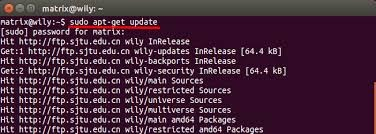
\includegraphics[width=1\textwidth]{../figures/1aptupdate.jpg} 
\caption{sudo apt-get update}
\label{update}
\end{center}
\end{figure}
Pada Gambar \ref{update} menjelaskan tentang untuk memperbaharui daftar paket.
\begin{figure}[h]
\begin{center}
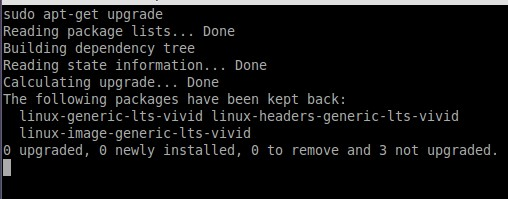
\includegraphics[width=1\textwidth]{../figures/1aptupgrade.jpg} 
\caption{sudo apt-get upgrade}
\label{upgrade}
\end{center}
\end{figure}

Pada Gambar \ref{upgrade} menjelaskan tentang untuk memperbaharui perangkat lunak sistem.
\item Proses Instalasi PIP di linux \\
Proses instalasi PIP di linux sangat sederhana karena hanya melakukan command satu perintah di Terminal.\\
\begin{figure}[h]
\begin{center}
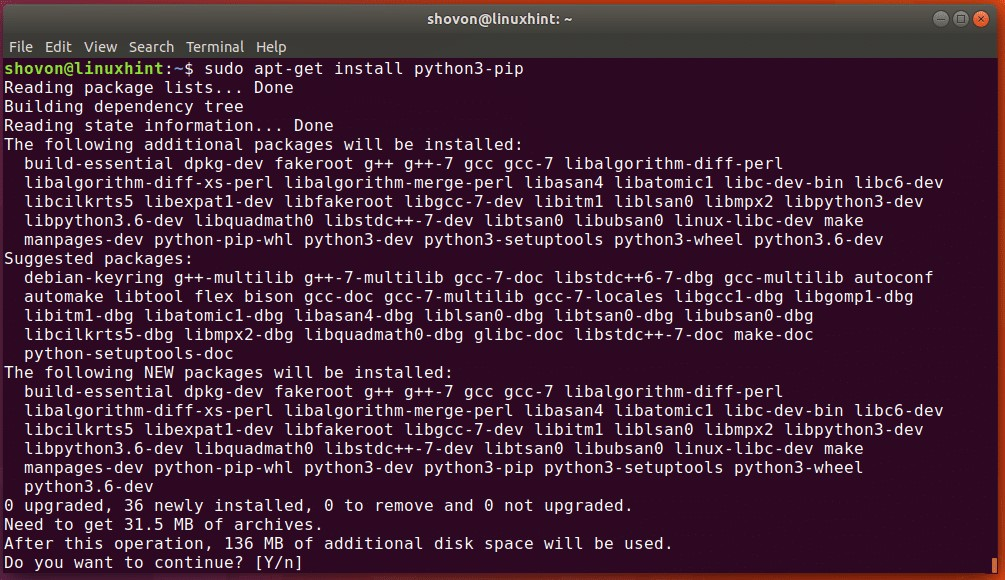
\includegraphics[width=1\textwidth]{../figures/1aptinstal.jpg} 
\caption{sudo apt-get update}
\label{instal}
\end{center}
\end{figure}
Pada Gambar \ref{instal} menjelaskan tentang proses melakukan instalasi pyhton.
\item Verifikasi PIP \\
Proses ini untuk menverifikasi apakah pip dan semua dependensi sudah terinstal atau belum agar dapat berjalan dengan optimal.\\
\begin{figure}[h]
\begin{center}
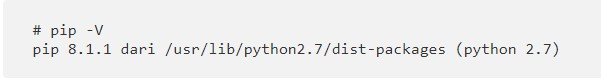
\includegraphics[width=1\textwidth]{../figures/1aptver.jpg} 
\caption{Pip -V}
\label{versi}
\end{center}
\end{figure}

Pada Gambar \ref{versi} menjelaskan tentang untuk menunjukkan versi pip yang telah diinstal.
\subsection{Instalasi PIP di Linux}
Pada umumnya perangkat python merupakan perangkat lunak yang termasuk di dalam disribusi Linux. Untuk linux distribusi slackware digunakan Python versi 2.4, yang terdapat pada CD I direktori/slackware/d. Menggunakan Toolkit untuk melakukan installasi paket di slackware adalah installpkg, berikut langkah instalasinya.\\
\item  mount/mnt/cdrom\\
\item  cd/mnt/cdrom/slackware/d\\
\item  installpkg python-2.4.1-i486-1tgz\\
\\
Python adalah menyediakan modus interaktif yang sangat berguna dalam melakukan latihan dan tes kode. Untuk menulis kode dalam modus interaktif dilakukan dengan memanggil toolkit python pada shell Linux. \\
\item  python\\
\item Python 2.4.1 (1, Apr 10 2005, 22:30:36) \\
\item GCC 3.3.5 on linux2 \\
\item Type "help", "copyright", "credits" or "license" \\
\item for more information.\\
\item  >>>\\
 Tanda “>>>” merupakan suatu prompt dalam modus interaktif Python, selanjutnya Python siap menerima input kode yang dimasukkan.\\

\section{Perintah Dasar PIP}
\subsection{Perintah Bantuan dalam PIP}
Berikut beberapa fungsi yang dapat membantu pengguna ketika dalam menggunakan PIP, antara lain :
\subsubsection{Help}
\begin{figure}[h]
\begin{center}
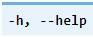
\includegraphics[width=1\textwidth]{../figures/1help.jpg}
\caption{Fungsi Help}
\label{FungsiHelp}
\end{center}
\end{figure}
Pada Gambar \ref{FungsiHelp} menjelaskan bahwa salah satu fungsi dalam PIP yang dapat menunjukkan bantuan.
\subsubsection{Version}
\begin{figure}[h]
\begin{center}
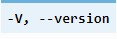
\includegraphics[width=1\textwidth]{../figures/1versi.jpg} 
\caption{Fungsi Version}
\label{fungsiversi}
\end{center}
\end{figure}
Pada Gambar \ref{fungsiversi} menjelaskan tentang salah satu fungsi pada PIP yang dapat menunjukkan versi PIP yang kita gunakan.
\subsubsection{Cache}
\begin{figure}[h]
\begin{center}
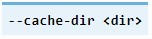
\includegraphics[width=1\textwidth]{../figures/1cache.jpg} 
\caption{Fungsi cache}
\label{fungsicache}
\end{center}
\end{figure}
Pada Gambar \ref{fungsicache} menjelaskan tentang salah satu fungsi pada PIP yang dapat mmenyimpan data cache ke direktori %<dir>
\subsubsection{No Cache}
\begin{figure}[h]
\begin{center}
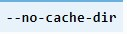
\includegraphics[width=1\textwidth]{../figures/1nocache.jpg} 
\caption{Fungsi NoCache}
\label{fungsinocache}
\end{center}
\end{figure}
Pada Gambar \ref{fungsinocache} menjelaskan tentang salah satu fungsi pada PIP untuk menonaktifkan cache
\subsection{Dasar PIP}
Ada beberapa aturan dalam menangani penggunaan string python yang dapat diandalkan :
\item Tanda kutip tunggal (') atau tanda kuutip ganda (")
\item Apabila dalam penggunaan suatu string terdapat karakter kutip tunggal (') penulisannya diapit kutip ganda (")
\item Apabila dalam penggunaan suatu string terdapat karakter kutip tunggal (") penulisannya diapit kutip ganda (')
\subsection{Perintah Dasar PIP}
Ada beberapa sintaks dasar dalam pemrograman python.
1.	Insialisasi variable. Inisialisasi variable atau statement penugasan adalah sintaks dasar dalam python, contohnya a = 2. Angka 2 adalah identitas dari variable a. Selain itu, ada juga yang dinamakan statement multi baris yang ditandai dengan beberapa baris yang terdapat symbol slash (/"). Ada pula yang dinamakan statement tanda kurung '[]','{}','()" tanpa ada slash (/")
2.	Baris dan indentasi. Kode blok yang digunakan di python menggunakan spasi (indentasi). Jumlah spasi setiap baris yang ada dalam satu blok harus sama dan sesuai.
3.	Tanda kutip dalam python. Python menggunakan tanda kutip ('), (""), ('"), ("") untuk menandai string.
4.	Komentar di python. Tidak seperti Bahasa pemrograman lain yang umumnya menandai komentar denga symbol backslash (\"). Di pemrograman python, komentar di tanadi denga symbol tetagar (\#).
\subsection{Perintah Dasar PIP}
Perintah-perintah dasar pip
Disini saya akan menjelaskan tentang instalasi package
1.	Untuk perintah instalasi package menggunakan perintah $pip install <nama-package>
2.	Bisa menambahkan versi sesuai yang diinginkan dibelakangnya contohnya $pip install <nama-package>=2.0.1
3.	Sebagai contohnya, disini akan menginstal pafy dengan menggunakan perintah $ pip install pafy
4.	Lalu uji dengan perintah $python -c import pafy
5.	Dan selesai..

\section{Contoh Penggunaan PIP}
\subsection{Contoh penggunaan PIP} 
Contoh Pengguaan pip dalam Proses enkripsi dan deskripsi suatu file dengan algoritma Huffman di implementasikan dalam bahasa python.
\item	Fungsi main
Digunakan perintah python [compress/decompress] [filename] untuk argumen “compress” untuk mengenkripsi dan memampatkan file dan argumen decompress untuk membuka kembali menjadi file.
\item	Fungsi ENCODE
Hasil file yang di enkripsi adalah Namafile+’Compressed.txt’.
\item	Fungsi DECODE
Hasil file adalah NamaFile + ’decompressed.txt’.
\subsection{Contoh penggunaan PIP}
Kita dapat melakukan install package-package yang dibundel dengan file berekstensi whl melalui PIP,wheel adalah format arsip yang digunakan untuk mempercepat melakukan penginstalan package. Setelah melakukan penginstalan wheel, lakukan penginstalan paket dengan menggunakan perintah pip install nipype-0.10.0-py2-none-any.whl . Untuk menampilkan package-package yang telah di install gunakan perintah pip list dan untuk menguninstall package lakukan dengan perintah pip uninstall <nama-package>.
\subsection{Instalasi Package Sekaligus}
Pada PIP, kita dapat melakukan penginstalan package sekaligus lebih dari satu package dan  kita tdiak perlu repot untuk menginstal satu per satu package. Pada PIP, untuk menginstal package sekaligus menggunakan requirement.txt, dimana kita melakukan list package yang akan di list dan dimasukkan dalam requirement.txt tersebut. Lalu kita ketikkan perintah
\begin{figure}[h]
\begin{center}
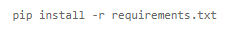
\includegraphics[width=1\textwidth]{../figures/1requre.png}
\caption{Perintah Instal Package Sekaligus}
\label{1require} 
\end{center}
\end{figure}
Pada gambar \ref{1require} menjelaskan tentang bagaimana cara instal package sekaligus dalam satu waktu.
\end{itemize}
\end{document}